%%% BEN 5' %%%

\section{Allgemeine Grundlagen}

\subsection{Die Hyperfeinstruktur}



\begin{frame}
\frametitle{Hyperfeinstruktur-Auspaltung}
  HFS
  
\setbeamerfont{myfont}{size*=45}
\usebeamerfont{myfont}

  \begin{figure}
    \centering
    \def\svgwidth{0.45\textwidth}
    \input{../img/termschema.pdf_tex}
    %\caption{Termschemata der beiden Rubidiumisotope:
    %Feinstruktur, Hyperfeinstruktur und Zeeman-Aufspaltung der D$_1$-Linie im äußeren Magnetfeld.}
    \label{img:termschema}
\end{figure}
\end{frame}




%%% MORITZ 2.5' %%%

\subsection{Laser}



\begin{frame}
\frametitle{Laser - Aufbau}

\setbeamerfont{myfont}{size*=80}
\usebeamerfont{myfont}
\begin{figure}
    \centering
    \def\svgwidth{\textwidth}
    \input{../img/aufbauLaser.pdf_tex}
    \caption{Aufbau zur Messung der $P$-$I$-Kennlinie der Laserdiode.}
\end{figure}

\end{frame}






\begin{frame}
\frametitle{$P$-$I$-Kennlinie}

\begin{figure}[H]
\begin{center}
  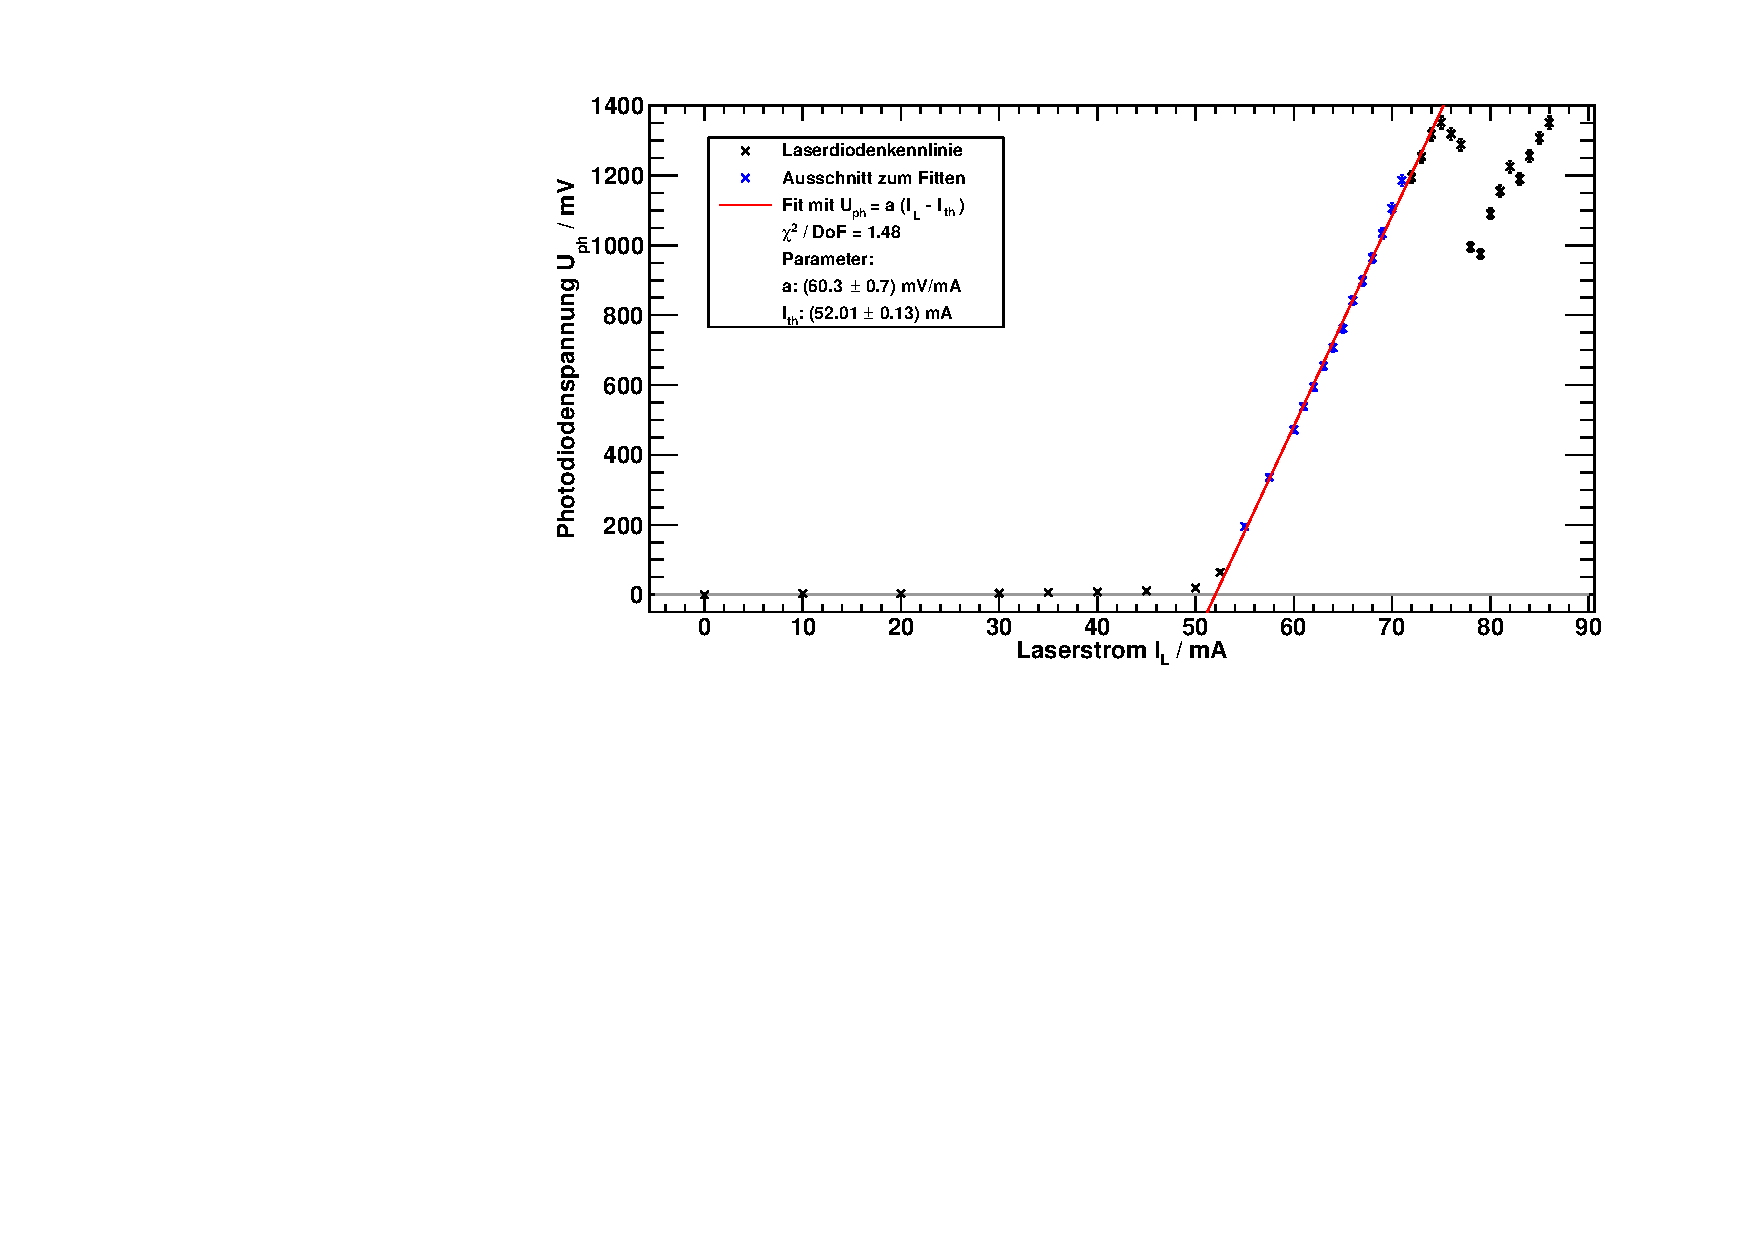
\includegraphics[width=\textwidth]{../img/diodenkennlinie.pdf}
  \caption{$P$-$I$-Kennlinie der im Versuch verwendeten Laserdiode.}
\end{center}
\end{figure}

\end{frame}


\begin{frame}
\frametitle{Laser - Aufbau}

\setbeamerfont{myfont}{size*=80}
\usebeamerfont{myfont}
\begin{figure}
    \centering
    \def\svgwidth{\textwidth}
    \input{../img/aufbauEtalon.pdf_tex}
    \caption{Aufbau zur Identifikation von Modensprüngen der Laserdiode.}
\end{figure}

\end{frame}


\begin{frame}
\frametitle{Etalon - Modensprung}

\begin{figure}[H]
\begin{center}
  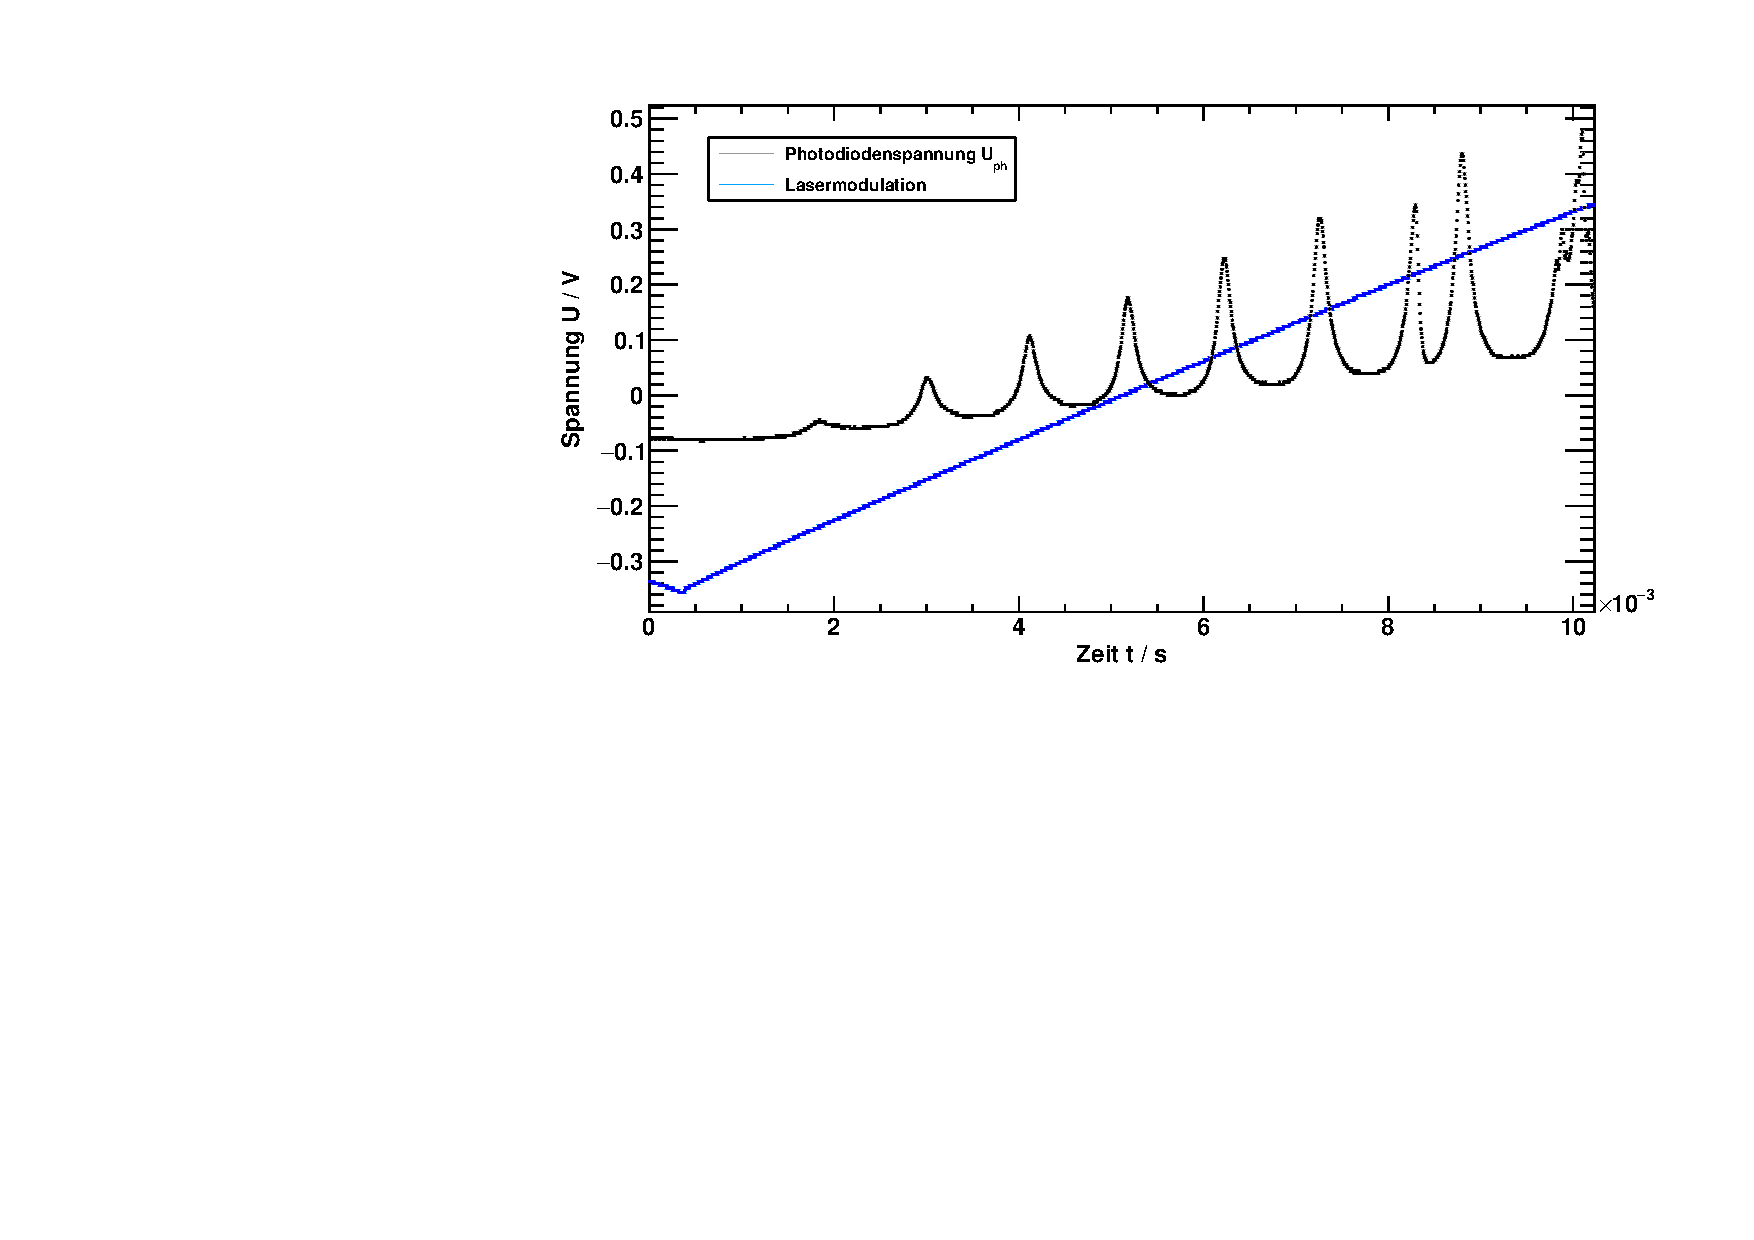
\includegraphics[width=\textwidth]{../img/up-etalon_zoom.pdf}
  \caption{caption.}
\end{center}
\end{figure}

\end{frame}

